% !TeX spellcheck = da_DK
%implementing document formatting:
\documentclass[a4paper,11pt,fleqn,dvipsnames,oneside,openright,oldfontcommands]{memoir} 	% Openright aabner kapitler paa hoejresider (openany begge)

\usepackage{xfrac}
\usepackage{booktabs}
\usepackage[table,xcdraw]{xcolor}

%%%%%%%%% Indsat random
%makes it possible to refer to the name of a chapter rather than just the number.
\usepackage{nameref}
\usepackage{pdfpages}
\usepackage{marvosym}
\usepackage{setspace}
\usepackage{graphicx} % For at sætte 2 billeder ved siden af hinanden

%package for writing program code in latex
\usepackage{listings}
%%%%%%%%%%%%%%%%%%%%%%

% ¤¤ Oversaettelse og tegnsaetning ¤¤ %
\usepackage[T1]{fontenc}					% Output-indkodning af tegnsaet (T1)
\usepackage[danish]{babel}					% Dokumentets sprog
\usepackage[utf8]{inputenc}					% Input-indkodning af tegnsaet (UTF8)
\usepackage{ragged2e,anyfontsize}			% Justering af elementer
\usepackage{fixltx2e}						% Retter forskellige fejl i LaTeX-kernen			
\usepackage{gensymb}						% Nu kan der skrices procent tegn med \degree				
				
																							
% ¤¤ Figurer og tabeller (floats) ¤¤ %
\usepackage{graphicx} 						% Haandtering af eksterne billeder (JPG, PNG, EPS, PDF)
%\usepackage{eso-pic}						% Tilfoej billedekommandoer paa hver side
\usepackage{wrapfig}						% Indsaettelse af figurer omsvoebt af tekst. \begin{wrapfigure}{Placering}{Stoerrelse}
\usepackage{multirow}                		% Fletning af raekker og kolonner (\multicolumn og \multirow)
\usepackage{multicol}         	        	% Muliggoer output i spalter
\usepackage{rotating}						% Rotation af tekst med \begin{sideways}...\end{sideways}
\usepackage{colortbl} 						% Farver i tabeller (fx \columncolor og \rowcolor)
\usepackage{xcolor}							% Definer farver med \definecolor. Se mere: http://en.wikibooks.org/wiki/LaTeX/Colors
\usepackage{flafter}						% Soerger for at floats ikke optraeder i teksten foer deres reference
\let\newfloat\relax 						% Justering mellem float-pakken og memoir
\usepackage{float}							% Muliggoer eksakt placering af floats, f.eks. \begin{figure}[H]
\usepackage{array,booktabs,xcolor,longtable} % kan lave \hdashline i tabellertabe
\usepackage{arydshln}
\usepackage{tabu}
\usepackage{epstopdf} 						% Muligoer brugen af eps filer i latex

	
	
% ¤¤ Matematik mm. ¤¤
\usepackage{amsmath , amsthm , amsfonts , amssymb, float, stmaryrd} 		% Avancerede matematik-udvidelser
%\usepackage{mathtools}						% Andre matematik- og tegnudvidelser
\usepackage{textcomp}                 		% Symbol-udvidelser (f.eks. promille-tegn med \textperthousand )
\usepackage{rsphrase}						% Kemi-pakke til RS-saetninger, f.eks. \rsphrase{R1}
\usepackage[version=3]{mhchem} 				% Kemi-pakke til flot og let notation af formler, f.eks. \ce{Fe2O3}
\usepackage{siunitx}						% Flot og konsistent praesentation af tal og enheder med \si{enhed} og \SI{tal}{enhed}
\sisetup{output-decimal-marker = {,}}		% Opsaetning af \SI (DE for komma som decimalseparator) 

% ¤¤ Referencer og kilder ¤¤ %
\usepackage[danish]{varioref}				% Muliggoer bl.a. krydshenvisninger med sidetal (\vref)
\usepackage[numbers]{natbib}				% Udvidelse med naturvidenskabelige citationsmodeller
%%\usepackage[sort&compress,square,comma,numbers]{natbib}
\newcommand{\citer}[1]{\citeauthor{#1},~\citeyear{#1}~\cite{#1}}

%\DeclareRobustCommand{\citer}[1]{\citeauthor{#1},~\citeyear{#1}~\cite{#1}}
											% citere i teksten: "Et studie af 'forfatter', 'år' [kilde#] viser..."
%\usepackage{xr}							% Referencer til eksternt dokument med \externaldocument{<NAVN>}
%\usepackage{glossaries}					% Terminologi- eller symbolliste (se mere i Daleifs Latex-bog)
\usepackage{lastpage}					% Gør det mulig at refere til sidste side 

% ¤¤ Misc. ¤¤ %
\usepackage{listings}						% Placer kildekode i dokumentet med \begin{lstlisting}...\end{lstlisting}
\usepackage{lipsum}							% Dummy text \lipsum[..]
\usepackage[shortlabels]{enumitem}			% Muliggoer enkelt konfiguration af lister
\usepackage{pdfpages}						% Goer det muligt at inkludere pdf-dokumenter med kommandoen \includepdf[pages={x-y}]{fil.pdf}	
\pdfoptionpdfminorversion=6					% Muliggoer inkludering af pdf dokumenter, af version 1.6 og hoejere
\pretolerance=2500 							% Justering af afstand mellem ord (hoejt tal, mindre orddeling og mere luft mellem ord)


% Kommentarer og rettelser med \fxnote. Med 'final' i stedet for 'draft' udloeser hver note en error i den faerdige rapport.
\usepackage[footnote,final,danish,silent,nomargin]{fixme}		


%%%% CUSTOM SETTINGS %%%%

% ¤¤ Marginer ¤¤ %
\setlrmarginsandblock{3.0cm}{2.5cm}{*}		% \setlrmarginsandblock{Indbinding}{Kant}{Ratio}
\setulmarginsandblock{2.5cm}{3.0cm}{*}		% \setulmarginsandblock{Top}{Bund}{Ratio}
\checkandfixthelayout 						% Oversaetter vaerdier til brug for andre pakker

%	¤¤ Afsnitsformatering ¤¤ %
\setlength{\parindent}{0mm}           		% Stoerrelse af indryk
\setlength{\parskip}{3mm}          			% Afstand mellem afsnit ved brug af double Enter
\linespread{1,1}							% Linie afstand



% ¤¤ Indholdsfortegnelse ¤¤ %
\setsecnumdepth{subsection}		 			% Dybden af nummerede overkrifter (part/chapter/section/subsection)
\maxsecnumdepth{subsection}					% Dokumentklassens graense for nummereringsdybde
\settocdepth{section} 					% Dybden af indholdsfortegnelsen

% ¤¤ Lister ¤¤ %
\setlist{
  topsep=0pt,								% Vertikal afstand mellem tekst og listen
  itemsep=-1ex,								% Vertikal afstand mellem items
} 

%hyperlinks in the tabel of contents - comment this out before the report is printed.
\usepackage{hyperref}
\hypersetup{
	bookmarks = true,  % Show 'bookmark'-frame in pdf.
	colorlinks = true, % True = colored links, False = framed links.
	citecolor = black,  % Link color for references.
	linkcolor = black,  % Link color in table of contents.
	urlcolor = black,   % Link color for extern URLs.
}

% ¤¤ Opsaetning af figur- og tabeltekst ¤¤ %
\usepackage{caption}
\usepackage{subcaption}
\captionnamefont{\small\bfseries\itshape}	% Opsaetning af tekstdelen ('Figur' eller 'Tabel')
\captiontitlefont{\small}					% Opsaetning af nummerering
\captiondelim{. }							% Seperator mellem nummerering og figurtekst
\hangcaption								% Venstrejusterer flere-liniers figurtekst under hinanden
%\captionwidth{0.9\textwidth}					% Bredden af figurteksten
\setlength{\belowcaptionskip}{0pt}			% Afstand under figurteksten
\captionsetup[figure]{labelfont={bf,it},font={it}} % sætter nummer til fed og kursis. Resten til fed + skriften er mindre end resten
\captionsetup[table]{labelfont={bf,it},font={it}} 


% ¤¤ Opsaetning af listings ¤¤ %

\definecolor{commentGreen}{RGB}{34,139,24}
\definecolor{stringPurple}{RGB}{208,76,239}

\lstset{language=Matlab,					% Sprog
	basicstyle=\ttfamily\scriptsize,		% Opsaetning af teksten
	keywords={for,if,while,else,elseif,		% Noegleord at fremhaeve
			  end,break,return,case,
			  switch,function},
	keywordstyle=\color{blue},				% Opsaetning af noegleord
	commentstyle=\color{commentGreen},		% Opsaetning af kommentarer
	stringstyle=\color{stringPurple},		% Opsaetning af strenge
	showstringspaces=false,					% Mellemrum i strenge enten vist eller blanke
	numbers=left, numberstyle=\tiny,		% Linjenumre
	extendedchars=true, 					% Tillader specielle karakterer
	columns=flexible,						% Kolonnejustering
	breaklines, breakatwhitespace=true,		% Bryd lange linjer
}

% ¤¤ Navngivning ¤¤ %
\addto\captionsdanish{
	\renewcommand\appendixname{Appendiks}
	\renewcommand\contentsname{Indholdsfortegnelse}	
	\renewcommand\appendixpagename{Appendiks}
	\renewcommand\appendixtocname{Appendiks}
	\renewcommand\cftchaptername{\chaptername~}				% Skriver "Kapitel" foran kapitlerne i indholdsfortegnelsen
	\renewcommand\cftappendixname{\appendixname~}			% Skriver "Appendiks" foran appendiks i indholdsfortegnelsen
}

% ¤¤ Kapiteludssende ¤¤ %
\definecolor{numbercolor}{gray}{0.7}		% Definerer en farve til brug til kapiteludseende
\newif\ifchapternonum

\makechapterstyle{jenor}{					% Definerer kapiteludseende frem til ...
	\renewcommand\beforechapskip{0pt}
	\renewcommand\printchaptername{}
	\renewcommand\printchapternum{}
	\renewcommand\printchapternonum{\chapternonumtrue}
	\renewcommand\chaptitlefont{\fontfamily{pbk}\fontseries{db}\fontshape{n}\fontsize{20}{35}\selectfont\raggedright}
	\renewcommand\chapnumfont{\fontfamily{pbk}\fontseries{m}\fontshape{n}\fontsize{0.35in}{0in}\selectfont\color{black}}
	\renewcommand\printchaptertitle[1]{%
		\noindent
		\ifchapternonum
		\begin{tabularx}{\textwidth}{X}
			{\let\\\newline\chaptitlefont ##1\par} 
		\end{tabularx}
		\par\vskip-2.5mm\hrule
		\else
		\begin{tabularx}{\textwidth}{Xl}
			{\parbox[b]{\linewidth}{\chaptitlefont ##1}} & \raisebox{-5pt}{\chapnumfont \thechapter}
		\end{tabularx}
		\par\vskip2mm\hrule
		\fi
	}
}											% ... her

\chapterstyle{jenor}						% Valg af kapiteludseende - Google 'memoir chapter styles' for alternativer

% ¤¤ Sidehoved ¤¤ %

\makepagestyle{AAU}							% Definerer sidehoved og sidefod udseende frem til ...
\makepsmarks{AAU}{%
	\createmark{chapter}{left}{shownumber}{}{. \ }
	\createmark{section}{right}{shownumber}{}{. \ }
	\createplainmark{toc}{both}{\contentsname}
	\createplainmark{lof}{both}{\listfigurename}
	\createplainmark{lot}{both}{\listtablename}
	\createplainmark{bib}{both}{\bibname}
	\createplainmark{index}{both}{\indexname}
	\createplainmark{glossary}{both}{\glossaryname}
}
\nouppercaseheads											% Ingen Caps oenskes

\makeevenhead{AAU}{Gruppe 5406}{}{\leftmark}				% Definerer lige siders sidehoved (\makeevenhead{Navn}{Venstre}{Center}{Hoejre})
\makeoddhead{AAU}{\rightmark}{}{Aalborg Universitet}		% Definerer ulige siders sidehoved (\makeoddhead{Navn}{Venstre}{Center}{Hoejre})
\makeevenfoot{AAU}{\thepage}{}{}							% Definerer lige siders sidefod (\makeevenfoot{Navn}{Venstre}{Center}{Hoejre})
\makeoddfoot{AAU}{}{}{\thepage}								% Definerer ulige siders sidefod (\makeoddfoot{Navn}{Venstre}{Center}{Hoejre})
\makeheadrule{AAU}{\textwidth}{0.5pt}						% Tilfoejer en streg under sidehovedets indhold
\makefootrule{AAU}{\textwidth}{0.5pt}{1mm}					% Tilfoejer en streg under sidefodens indhold

\copypagestyle{AAUchap}{AAU}								% Sidehoved for kapitelsider defineres som standardsider, men med blank sidehoved
\makeoddhead{AAUchap}{}{}{}
\makeevenhead{AAUchap}{}{}{}
\makeheadrule{AAUchap}{\textwidth}{0pt}
\aliaspagestyle{chapter}{AAUchap}							% Den ny style vaelges til at gaelde for chapters
% ... her

\pagestyle{AAU}												% Valg af sidehoved og sidefod


%%%% CUSTOM COMMANDS %%%%

% ¤¤ Billede hack ¤¤ %
\newcommand{\figur}[4]{
		\begin{figure}[H] \centering
			\includegraphics[width=#1\textwidth]{billeder/#2}
			\caption{#3}\label{#4}
		\end{figure} 
}

% ¤¤ Specielle tegn ¤¤ %
\newcommand{\decC}{^{\circ}\text{C}}
\newcommand{\dec}{^{\circ}}
\newcommand{\m}{\cdot}


%%%% ORDDELING %%%%

\hyphenation{}

%%%%Fra engelsk til dansk i \autoref{•} %%%%
\renewcommand{\figureautorefname}{Figur}
\renewcommand{\sectionautorefname}{Afsnit}
\renewcommand{\subsectionautorefname}{Afsnit}
\renewcommand{\subsubsectionautorefname}{Afsnit}
\renewcommand{\tableautorefname}{Tabel}
\renewcommand{\appendixautorefname}{Appendiks}
\renewcommand{\equationautorefname}{Ligning}
\renewcommand{\itemautorefname}{Punkt}
\renewcommand{\chapterautorefname}{Kapitel}
\raggedbottom
%Figure references:
\newcommand{\figref}[1]{figur~\ref{#1}}

%Figure references after full stop/period:
\newcommand{\Figref}[1]{Figur~\ref{#1}}

%Table references:
\newcommand{\tabref}[1]{tabel~\ref{#1}}

%Table references after full stop/period:
\newcommand{\Tabref}[1]{Tabel~\ref{#1}}

%Appendix references:
\newcommand{\appref}[1]{appendiks~\ref{#1}}

%Appendix references after full stop/period:
\newcommand{\Appref}[1]{Appendiks~\ref{#1}}

%Section references:
\newcommand{\secref}[1]{afsnit~\ref{#1}}

%Section references:
\newcommand{\Secref}[1]{Afsnit~\ref{#1}}

%chapter references: 
\newcommand{\chapref}[1]{kapitel~\ref{#1}}

%chapter references: 
\newcommand{\Chapref}[1]{Kapitel~\ref{#1}}


%Units:
%inserting '\omit' before '{\put' prior ot final compile will fix allignment (and generate errors)
\newcommand{\unit}[1]{{\put(300,0){$\hfill\left[\: #1 \:\right]$}}}

%Text:
\newcommand{\tx}[1]{\text{#1}}

%Equation references:
%1 equation:
\renewcommand{\eqref}[1]{ligning~(\ref{#1})}
%2 equations:
\newcommand{\eqrefTwo}[2]{ligning~(\ref{#1}) og (\ref{#2})}
%3 equations:
\newcommand{\eqrefThree}[3]{ligning~(\ref{#1}), (\ref{#2}) og (\ref{#3})}
%4 equations:
\newcommand{\eqrefFour}[4]{ligning (\ref{#1}), (\ref{#2}), (\ref{#3}) og (\ref{#4})}
%5 equations:
\newcommand{\eqrefFive}[5]{ligning (\ref{#1}), (\ref{#2}), (\ref{#3}), (\ref{#4}) og (\ref{#5})}


%Equation references after full stop/period:
%1 equation:
\newcommand{\Eqref}[1]{Ligning~(\ref{#1})}
%2 equations:
\newcommand{\EqrefTwo}[2]{Ligning~(\ref{#1}) og (\ref{#2})}
%3 equations:
\newcommand{\EqrefThree}[3]{Ligning~(\ref{#1}), (\ref{#2}) og (\ref{#3})}
%4 equations:
\newcommand{\EqrefFour}[4]{Ligning (\ref{#1}), (\ref{#2}), (\ref{#3}) og (\ref{#4})}
%5 equations:
\newcommand{\EqrefFive}[5]{Ligning (\ref{#1}), (\ref{#2}), (\ref{#3}), (\ref{#4}) og (\ref{#5})}
\begin{document}

%numbers the pages with Roman numeral - starts from "i":
\frontmatter
\clearpage
\thispagestyle{empty}

%\begin{figure}[H]
%	\raggedleft
%		
\includegraphics[width=0.2\textwidth]{figures/aaulogo-da.png}
%\end{figure}


%\vspace*{\fill} 
%\begin{center}	
%	\begin{Huge}
%		P3 Projektrapport - efterår 2015\\
%		\vspace{5 mm}
%		\textbf{System til detektering af kropsbalance}\\
%		\vspace{3 mm}
%		Gruppe 375
%	\end{Huge}
%\end{center}
%\vspace*{\fill}

\begin{center}
	\vspace*{\baselineskip}
	\rule{\textwidth}{1.6pt}\vspace*{-\baselineskip}\vspace*{2pt} % Thick horizontal line
	\rule{\textwidth}{0.4pt}\\[\baselineskip] % Thin horizontal line
	
	{\huge Aktivitetsmåler til forebyggelse\\\hspace*{2ex} af fysisk inaktivitet hos børn \\[0.5\baselineskip] \large Projektrapport 4. semester}\\[0.2\baselineskip] % Title
	
	\rule{\textwidth}{0.4pt}\vspace*{-\baselineskip}\vspace{3.2pt} % Thin horizontal line
	\rule{\textwidth}{1.6pt}\\[\baselineskip] % Thick horizontal line
	\vspace*{5\baselineskip}
	\begin{figure}[H]
		\centering
		\begin{minipage}[c]{1\textwidth}
			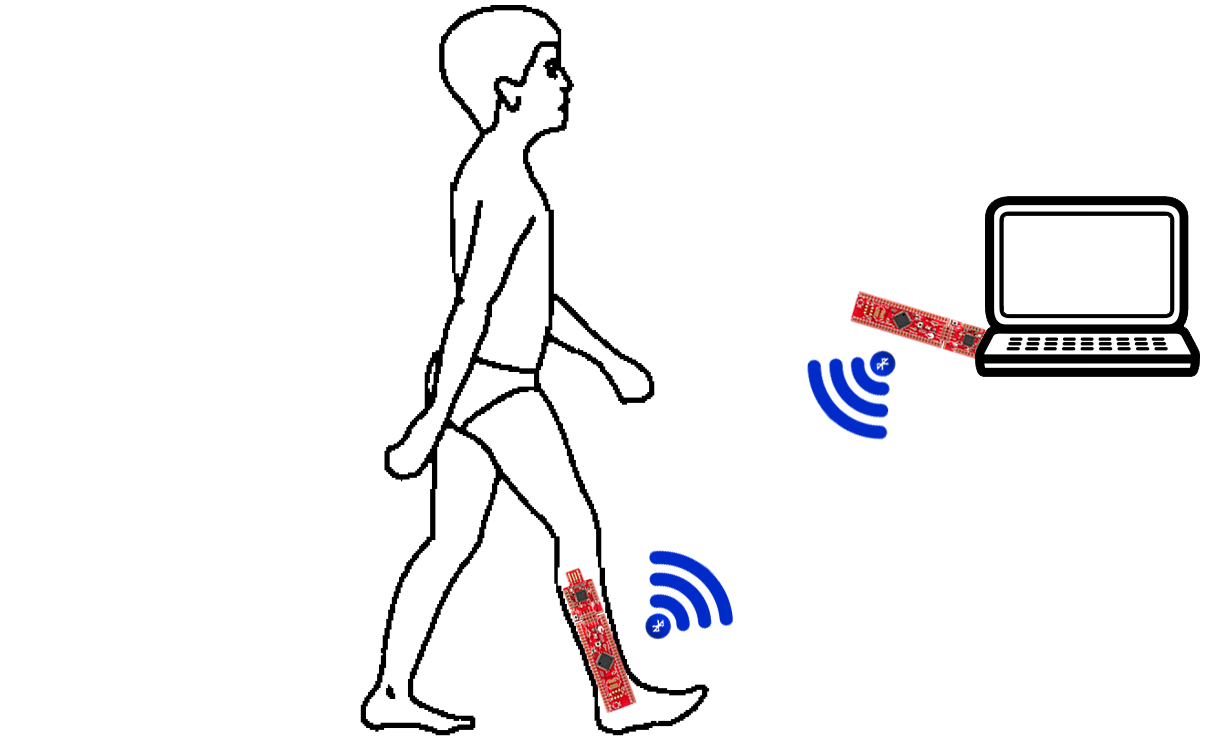
\includegraphics[width=.75\textwidth]{figures/forside2.PNG}
		\end{minipage}
		\hfill
	\end{figure}
	\vspace*{\fill}
	\scshape % Small caps
	{\Large Gruppe 4403\par}
	
	\vspace*{.8\baselineskip} % Whitespace between location/year and editors
	
	Aalborg Universitet,  01/02/2016 - 27/05/2016 \par % Location and year
\end{center} % Center all text
%{\color{white}X \\ X \\ X \\}

%\begin{center}
%	\textit{Gruppemedlemmer:}\\
%	Cecilie Sophie Rosenkrantz Topp, Frederik Skou Nielsen \\
%	Josefine Dam Gade, Line Sofie Hald, Morten Skaarup Larsen
%\end{center}
\begin{center}
	\line(1,0){400}
\end{center}

\clearpage
\thispagestyle{empty}
{\color{white}Dette giver en tom side}
\clearpage

%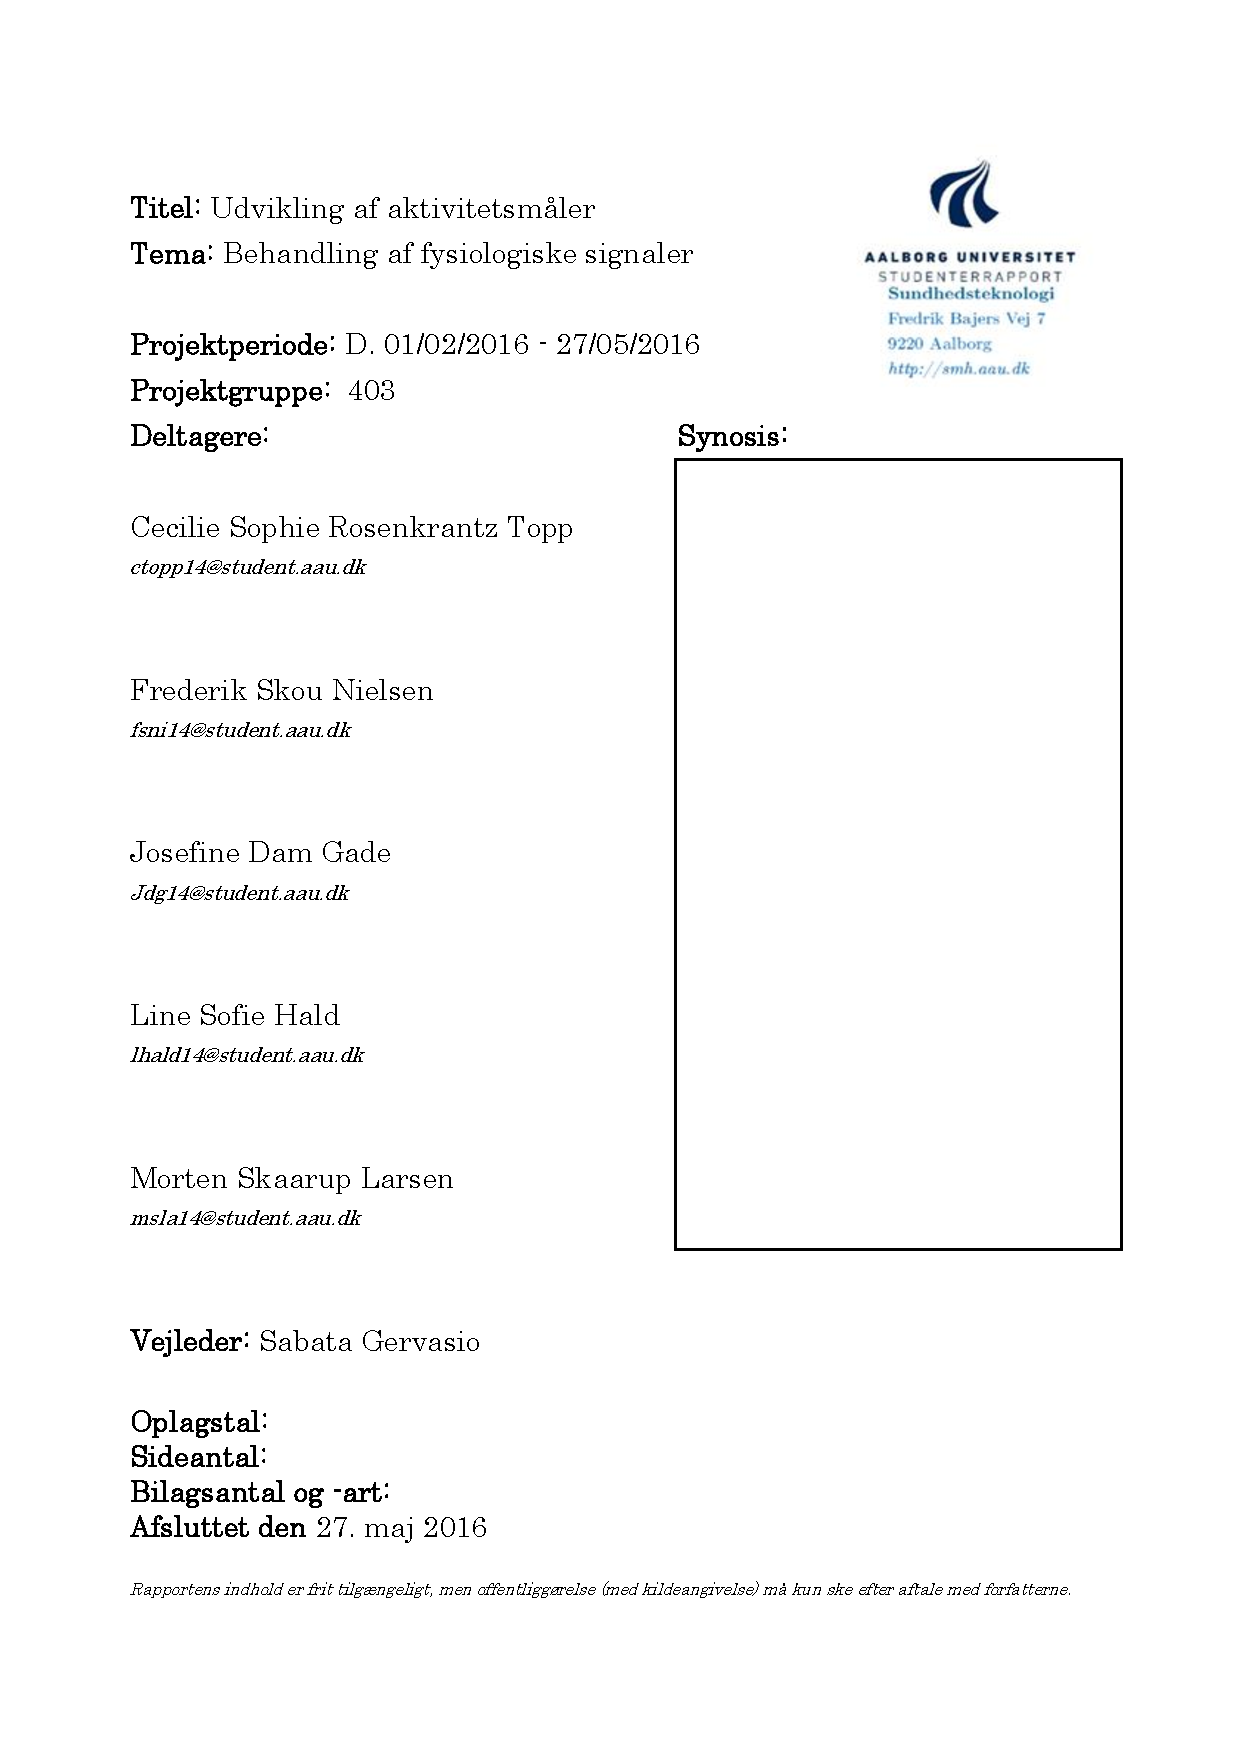
\includepdf[pages={1}]{rapportAfsnit/pFormaliteter/synopsis.pdf} \clearpage 
\include{rapportAfsnit/pFormaliteter/titelblad}

\chapter*{Forord og læsevejledning}\vspace{-.75cm}
% !TeX spellcheck = da_DK
\section*{Forord}
Denne rapport er udarbejdet som et 4. semesters projekt på bacheloruddannelsen i Sundhedsteknologi på Aalborg Universitet. Projektetperioden forløb fra 1. februar 2016 til 27. maj 2016. \\
Projektet tager udgangspunkt i studieordningen for bacheloruddannelsen i Sundhedsteknologi. Semesterets fokusområde er 'Behandling af fysiologiske signaler', hvor dette projekt tager udgangspunkt i projektforslaget 'Udvikling af aktivitetsmåler'. Formålet er blandt andet design, implementering og test af en prototype, der kan detektere fysisk aktivitet. Protoypen udvikles med henblik på at bestemme det fysiske aktivitetsniveau for børn i aldersgruppen 9-12 år. %Prototypen vil derfor involvere en dataopsamling fra analoge komponenter i form af et et accelerometer, et gyroskop og en pulssensor. Ydermere vil prototypen indeholde signal- og databehandling som muligøre digital visualisering på et grafisk brugerinterface.

%Projektet henvender sig til studerende på samme niveau eller andre interessere med et kendskab til basal analog og digital databehandling. \\
Der rettes en tak til vejleder Sabata Gervasio for et godt og lærerigt samarbejde under udarbejdelsen af denne rapport. Yderligere rettes der en tak til semesterkoordinater, John Hansen, for råd og vejledning til forståelse af semesterets nye mikrokontroller. 

\section*{Læsevejledning}
Projektet er opbygget af fem kapitler, en litteraturoversigt samt to bilag. Hvert kapitel og hovedafsnit indledes med et kursiv afsnit, som har til formål at vejlede læseren i henholdsvis kapitlets og hovedafsnittets indhold og sammenhæng i rapportens helhed.\\
Første kapitel består af en indledning og initierende problemstilling. Herefter er problemanalysen, der bearbejder den initierende problemstilling, hvilket leder frem til en problemformulering. Det tredje kapitel er problemløsning, hvori løsningsstrategi og essentielle teoretiske elementer beskrives. Yderligere indeholder kapitlet krav til prototypen og dets delelementer. Det efterfølgende kapitel består af design, implementering og test af systemets delementer samt en test af det samlede system. Afslutningsvis findes syntesen, indeholdende diskussion, konklusion og perspektivering.

Rapporten benytter Vancouver metoden til kildehenvisning. Alle benyttede kilder er at finde på side 91, hvor de er listet i numerisk rækkefølge. I tilfælde, hvor kilden befinder sig inden for punktum, tilhører denne kildehenvisning indholdet i den pågældende sætning. Er kildehenvisningen placeret efter punktummet i sætningen, tilhører kilden indholdet i det foregående afsnit. \\
Tabeller og figurer er nummereret efter deres respektive afsnit, hvorfor eksempelvis figur 1.1 er den første figur i kapitel 1.

Rapporten benytter forkortelser, hvor ordet skrives ud første gang det præsenteres med tilhørende forkortelse i parentes efter ordet. Efterfølgende vil denne forkortelse blive benyttet i resten af rapporten med undtagelse af overskrifter. 
\newpage

%the '*' allows the tableofcontents be excepted from the actual table of contents.
\tableofcontents* 

%numbers the pages with Arabic numeral - starts from 1.
\mainmatter

\chapter{Introduktion}\vspace{-.75cm}
%\input{rapportAfsnit/bInitierende\din fil martin}
\chapter{Problemanalyse}\vspace{-.75cm}
\section{Patientgruppe}
\textit{Følgende afsnit omhandler omfanget af lidelsen, knæartrose. Afsnittet redegør for patientomfanget, samt de forskellige disponeringsfaktorer, sammenkoblet med lidelsen. Ydermere vil patienternes patientforløb blive redegjort, hvoraf den sidste fase vil blive analyseret. Ovenstående vil danne grundlag for at klassificere en disponeret patientgruppe til knæalloplastik.}

Knæartrose er en lidelse hvor primært knæets ledbrusk gradvist bliver nedbrudt, og der sekundært sker forandringer i leddets knogler. Disse deformationer er irreversible, og kan dermed kan knæartrose kun afhjælpes og ikke kurreres. Lidelsen kan opdeles i en primær- og sekundær artrose. Dette adskilles per definition ved at den sekundære artrose indebærer tidligere skader, sygdom, inflammation, overvægt samt traume. Knæartrose er en tilstand hvis hyppigste symptomer indebærer smerter samt nedsat mobilitet hos den udsatte. Smerterne udtrykkes i forskellig grad, fra led igangsættende smerte til kronisk tilstedeværende smerte. Generelt for knæartrose, så forværres symptomerne i takt med graden af lidelsen øges. [Lægehåndbog, knæartrose]

Forekomsten af knæartrose er sammenholdt med en længere række faktorer, hvoraf man er i risiko for at være disponeret. Dette omhandler eksempelvis, overbelastning igennem arbejde og fritid, tidligere knæskader, arv, overvægt samt køn(kvinder)[Knæartrose – nationale kliniske retningslinjer, Sundhedsstyrrelsen]. Knæartrose er tilstede blandt 45\% af alle 80-årige blandt befolkningen. Dette tilfælde kan formodes at stige, som resultat af at der ses en tendens i samfundet, at levealderen i Danmark stiger. Dette er ikke det eneste tilfælde hvorfor prævalensen vil stige. En af de disponerende faktorer for knæartrose er overvægt, hvilket 47\% af den danske befolkning kan kategoriseres under. Ydermere stiger forekomsten af overvægt med alderen, hvilket forud for overvægten ligeledes er tilfældet for knæartrose. Overvægtige er disponeret for knæartrose med en relativ risiko på tre, hvoraf en kombination af ovenstående faktorer øger risikoen for lidelsen. [Patienthåndbogen, overvægt og fedme][lægehåndbog, overvægt][Patienthåndbog, slidgigt i knæ][Lægehåndbog, knæartrose]

Resultatet af en patients komplikationer kan medføre igangsættelse af et behandlingsforløb. Et behandlingsforløb for en patient med knæartrose består af flere faser, hvis mål er smertelindrende, mobilitetsforøgelse samt forebyggende. Generelt kan faserne opdeles i ikke-invasive og invasive metoder. Hvilken metode som afhjælper patienten afhænger heraf af graden af knæartrose. Første fase, hvis nødvendig, består af i en livsstilsændring, hvor en vægtreduktion samt øget fysiskaktivitet uden belastning, vil være fordelagtigt. Hvis dette ikke er tilstrækkeligt kan medicinsk behandling i form af smertelindrende medikamenter benyttes, enten som enkeltstående behandling eller sideløbende med fysioterapi. Hvis ikke, de ikke-invasive behandlingsmetoder afhjælper lidelsen i en grad hvor patienten er tilfreds, så bliver de invasive behandlingsmetoder taget til overvejelse. Overvejelsen heraf indebærer af den diagnosticerede grad af artrose, hvilket består af en sammenkobling af den kliniske vurdering, verificeret med forandringer i knæet opnået gennem røntgenbilleder. Baggrunden for at den kliniske vurdering skal verificeres forud for kirurgi, er at smerte fra hofte og ryg, kan projiceres til knæet.\\
Resultatet heraf er at patienten skal besidde svær slidgigt før patienten kvalificeres til kirurgi, og hermed en total knæalloplastik (TKA).  [Lægehåndbog, knæartrose][Knæartrose – nationale kliniske retningslinjer, Sundhedsstyrrelsen]

TKA er det sidst mulige behandlingsmetode for at udrede patientens komplikationer vedrørende knæartrose. Dette resulterede i at der i 2014 blev udført omtrent 9,8 tusinde TKA operationer, fordelt på førstegangs- og revisions operationer. [Dansk knæalloplastikregister, 2015] I takt med at TKA er den sidst mulige behandlingsmulighed, er operationstilfredshed en betydningsfuld problematik. I 2012 var 81-85\% af patienter der havde modtaget en TKA operation tilfredse, 8-11\%var decideret utilfredse, og resten var i tvivl eller til dels utilfreds. Dette er altså ensbetydende med at der potentielt er 19\% af alle operationer fra et patientøjemed som er ikke succesfulde. Resultatet heraf er at op mod 19\% ikke kan udredes fra deres smerter samt eventuel nedsatte mobilitet, trods alle behandlingsmetoder har været benyttet. [Knæartrose – nationale kliniske retningslinjer, Sundhedsstyrrelsen] Studiet af xxxxx har lavet en risikovurdering vedrørende kroniske smerter postoperativ TKA. Resultaterne betød at op mod 39\% af studiets patienter oplevede moderat til alvorlig smerte, 1 år postoperativt TKA. Ifølge International Association of Pain (IASP) er der tale om kroniske smerte, da dette er tilfældet ved vedvarende smerter tre måneder postoperativ. [Risk Assessment for Chronic Pain,link]. \\
Patientgruppen som postoperativt ikke er tilfredse er svært definerbar. Problematikken opstår i og med klassificeringen bag de potentielt 19-39\% udtilfredse patienter er vedrørende postoperative smerte samt mobilitet. Det kan forestilles at der blandt patienterne en forventningsfaktor, hvilket gør de kategoriserer dem selv som værende utilfreds, omend de rent faktisk har opnået en forbedring af både smerte og eller mobilitet. Det kan tænkes at forventningsfaktoren kan være medvirkende til kategorisere dem som værende utilfredse, som resultat af skuffelsen af ikke at fungere som et individ med et fuldt funktionsdygtigt knæ.  

Knæartrose er på bekostning af samfundets udvikling, en lidelse i vækst da den umiddelbare disponerede målgruppe er voksende. Resultatet heraf medfører at antallet af registrerede tilfælde vedrørende komplikationer sandsynligvis ligeledes vil stige, og der vil forekommer flere patienter med kroniske smerter postoperativt TKA, uden mulighed for yderligere alternativ behandling.


\textit{Kilderne er ikke sat ind - forstår stadig ikke mendeley. Når jeg opretter en manuel kilde - feks. web article, så kan jeg ikke vælge/se nogle citation key.}


\section{Smerte}

Smerte er blevet defineret som: “en ubehagelig sensorisk og emotionel oplevelse forbundet med egentligt eller potentiel skade af væv eller beskrevet i vendinger tilsvarende en lignende skade.” af den Internationale Association for Studiet af Smerte (Pain) (IASP) [Seminars in arthritis and rheumatism, Classification of Chronic Pain]. 
Selvom smerte normalt er en følelse man forsøger at undgå, er det en nødvendig del af vores overlevelse. Det fortæller kroppen om farer eller skader som der skal reageres på, som for eksempel at sætte hånden på en varm kogeplade. For ikke at blive slemt forbrændt og gøre skade på hånden, registrere nerver i huden en høj temperatur, som hånden skal fjernes fra. Nervesignalet sendes til central nervesystemet (CNS), hvor det først når rygmarven og lidt senere hjernen. Her skelnes der mellem smerte sensation og perception. Smerte sensation er information om smerte, som nerverne i hånden der registrere den skadelige temperatur. Smerte perceptionen sker først når nervesignalet når op til hjernen og denne modtager signalet og opfatter det som smerte. Sensationen af smerte kan i rygsøjlen aktivere en refleks der får musklerne i armen til at trække hånden væk fra varmen, inden hjernen når at registrere og opfatte den egentlige smerte. [Fundamentals of Human Anatomy and Physiologi 9th edition] Denne form for smerte er kategoriseret som øjeblikkelig smerte og defineres som “god” eller “nødvendig” smerte, da det hjælper kroppen med at undgå skader.

\subsection{Smerte typer}
Modsat denne “gode” smerte findes “dårlig” eller “unødvendig” smerte. Denne smerte kaldes også kronisk smerte, da den oftest er længere varende, ved at have været mere eller mindre konstant i mindst tre måneder [Seminars in arthritis and rheumatism]. Personer som lider af kronisk smerte har sjældent en synlig grund til at skulle føle smerte, og smerten er af den grund enten oplevet som smerte i indre organer eller psykogene smerter, som er forestillingen om en smerte. 
Ved organisk smerte skelnes der mellem to typer af smerte: nociceptisk og neuropatisk. Nociceptisksmerte er skade på væv og skyldes aktivering af nociceptorer, specielle nerveceller som er følsomme overfor temperatur ændringer, mekanisk stimuli eller kemiske ændringer i eller omkring celler, ved hjælp af specielle porte og pumper på nervecellerne. Nociceptorer findes i huden på kroppens overflader og i og omkring indre organer, og nociceptisksmerte opdeles i somatisk og viseral sensation. Somatisk smerte sensation og den øjeblikkelige og let placerbare smerte som at sætte hånden på en kogeplade. Viseral smerte sensation er mere besværlig at placere. Smerten er typisk ikke øjeblikkelig, men mere trykkende og langvarig. At have ondt i maven er et eksempel på viseral smerte. Nociceptisksmerte er oftest ikke årsag til kroniske smerter, med mindre smerterne bliver ved. 
Neuropatisk smerte er modsat nociceptisksmerte ikke skade på væv, men på nervesystemet selv, herunder nerver, rygmarv, nerve plexus eller hjernen. Dette kan skyldes direkte skade, sygdom som iskæmi eller sclerose, traume, diabetes, infektioner eller kræft. Smerten kan opleves som konstant og langvarig, hvor er typisk eksempel er fantom smerter, men kan også være lejlighedsvis som ved hyperalgesi, hvor almindelig berøring opfattes som smertefuldt. [Seminars in arthritis and rheumatism, Classification of Chronic Pain] 
Psykogene smerter er en forestillet opfattelse af smerte, og den mest besværlige at præcisere, idet der ikke er og muligvis aldrig har været en fysisk grund til smerten. Hos en person med psykogene smerter er hjernen fuldt overbevidst om, at den oplever fysiske smerter og lider der af. Smerten er udelukkende psykisk hos personen, men er af den grund ikke mindre virkelig, grundet smertes subjektive natur. [Seminars in arthritis and rheumatism]

\subsection{Problemet ved kronisk smerte og operationer}
Der findes således flere forskellige former for smerte, hvor kun nogle få er beskrevet her [Classification of Chronic Pain]. Alle kan de lede til kronisk smerte. Man ved derfor godt hvad der kan give kronisk smerte, hvordan smerten opfattes og hvor i kroppen den kommer fra. Men man ved endnu ikke hvorfor kronisk smerte opstår. Hvorfor føler kroppen fantom smerter fra et legeme som ikke er der? Hvorfor registrere hjernen smerte fra indre organer, når der intet er i vejen med dem? Et større problem opstår når man forsøger at behandle smerterne, med et ønske om at dæmpe eller helt fjerne smerterne, men smerterne fortsætter eller forværres. Sådan ses det i 20\% af tilfælde efter total knæalloplastik (TKA) operationer [Chronic Postoperative Pain After Primary and Revision Total Knee Arthroplasty]. Her oplever 19\% af patienter efter den primære operation, og 47\% af patienter efter revision af operationen oplever svære til uudholdelige smerter. Dette sker på trods af at der i hele Danmark udføres knæoperationer som alle signifikant overholder indikationerne for behandlingskvaliteten [Dansk Knæalloplastikregister, Årsrapport 2016]. De udførte TKA operationer må siges at være nær perfekte, men patienter oplever alligevel fortsatte smerter. 


\cleardoublepage
\chapter{Syntese}\vspace{-.75cm}
%\input{rapportAfsnit/../..}

\begingroup
\label{litteraturliste}
\raggedright
\bibliographystyle{unsrtnat}
\bibliography{kilder}
\endgroup
\begin{appendices}
%	\input{rapportAfsnit/qBilag/pilotforsoeg}
%	\input{rapportAfsnit/qBilag/MCU}
\end{appendices}

\end{document}
